\documentclass{tufte-book}

\hypersetup{colorlinks}% uncomment this line if you prefer colored hyperlinks (e.g., for onscreen viewing)

%%
% Book metadata
\title{Solutions to A Course In Combinatorics}
\author[Aakash Ghosh]{Aakash Ghosh}
\publisher{Summer 2022}

%%
% If they're installed, use Bergamo and Chantilly from www.fontsite.com.
% They're clones of Bembo and Gill Sans, respectively.
%\IfFileExists{bergamo.sty}{\usepackage[osf]{bergamo}}{}% Bembo
%\IfFileExists{chantill.sty}{\usepackage{chantill}}{}% Gill Sans

%\usepackage{microtype}

%%
% For nicely typeset tabular material
\usepackage{booktabs}

%%
% For graphics / images
\usepackage{graphicx}
\setkeys{Gin}{width=\linewidth,totalheight=\textheight,keepaspectratio}
\graphicspath{{graphics/}}

% The fancyvrb package lets us customize the formatting of verbatim
% environments.  We use a slightly smaller font.
\usepackage{fancyvrb}
\fvset{fontsize=\normalsize}

%%
% Prints argument within hanging parentheses (i.e., parentheses that take
% up no horizontal space).  Useful in tabular environments.
\newcommand{\hangp}[1]{\makebox[0pt][r]{(}#1\makebox[0pt][l]{)}}

%%
% Prints an asterisk that takes up no horizontal space.
% Useful in tabular environments.
\newcommand{\hangstar}{\makebox[0pt][l]{*}}

%%
% Prints a trailing space in a smart way.
\usepackage{xspace}

%%
% Some shortcuts for Tufte's book titles.  The lowercase commands will
% produce the initials of the book title in italics.  The all-caps commands
% will print out the full title of the book in italics.
\newcommand{\vdqi}{\textit{VDQI}\xspace}
\newcommand{\ei}{\textit{EI}\xspace}
\newcommand{\ve}{\textit{VE}\xspace}
\newcommand{\be}{\textit{BE}\xspace}
\newcommand{\VDQI}{\textit{The Visual Display of Quantitative Information}\xspace}
\newcommand{\EI}{\textit{Envisioning Information}\xspace}
\newcommand{\VE}{\textit{Visual Explanations}\xspace}
\newcommand{\BE}{\textit{Beautiful Evidence}\xspace}

\newcommand{\TL}{Tufte-\LaTeX\xspace}

% Prints the month name (e.g., January) and the year (e.g., 2008)
\newcommand{\monthyear}{%
	\ifcase\month\or January\or February\or March\or April\or May\or June\or
	July\or August\or September\or October\or November\or
	December\fi\space\number\year
}


% Prints an epigraph and speaker in sans serif, all-caps type.
\newcommand{\openepigraph}[2]{%
	%\sffamily\fontsize{14}{16}\selectfont
	\begin{fullwidth}
	\sffamily\large
	\begin{doublespace}
	\noindent\allcaps{#1}\\% epigraph
	\noindent\allcaps{#2}% author
	\end{doublespace}
	\end{fullwidth}
}

% Inserts a blank page
\newcommand{\blankpage}{\newpage\hbox{}\thispagestyle{empty}\newpage}

\usepackage{units}

% Typesets the font size, leading, and measure in the form of 10/12x26 pc.
\newcommand{\measure}[3]{#1/#2$\times$\unit[#3]{pc}}

% Macros for typesetting the documentation
\newcommand{\hlred}[1]{\textcolor{Maroon}{#1}}% prints in red
\newcommand{\hangleft}[1]{\makebox[0pt][r]{#1}}
\newcommand{\hairsp}{\hspace{1pt}}% hair space
\newcommand{\hquad}{\hskip0.5em\relax}% half quad space
\newcommand{\TODO}{\textcolor{red}{\bf TODO!}\xspace}
\newcommand{\na}{\quad--}% used in tables for N/A cells
\providecommand{\XeLaTeX}{X\lower.5ex\hbox{\kern-0.15em\reflectbox{E}}\kern-0.1em\LaTeX}
\newcommand{\tXeLaTeX}{\XeLaTeX\index{XeLaTeX@\protect\XeLaTeX}}
% \index{\texttt{\textbackslash xyz}@\hangleft{\texttt{\textbackslash}}\texttt{xyz}}
\newcommand{\tuftebs}{\symbol{'134}}% a backslash in tt type in OT1/T1
\newcommand{\doccmdnoindex}[2][]{\texttt{\tuftebs#2}}% command name -- adds backslash automatically (and doesn't add cmd to the index)
\newcommand{\doccmddef}[2][]{%
	\hlred{\texttt{\tuftebs#2}}\label{cmd:#2}%
	\ifthenelse{\isempty{#1}}%
		{% add the command to the index
			\index{#2 command@\protect\hangleft{\texttt{\tuftebs}}\texttt{#2}}% command name
		}%
		{% add the command and package to the index
			\index{#2 command@\protect\hangleft{\texttt{\tuftebs}}\texttt{#2} (\texttt{#1} package)}% command name
			\index{#1 package@\texttt{#1} package}\index{packages!#1@\texttt{#1}}% package name
		}%
}% command name -- adds backslash automatically
\newcommand{\doccmd}[2][]{%
	\texttt{\tuftebs#2}%
	\ifthenelse{\isempty{#1}}%
		{% add the command to the index
			\index{#2 command@\protect\hangleft{\texttt{\tuftebs}}\texttt{#2}}% command name
		}%
		{% add the command and package to the index
			\index{#2 command@\protect\hangleft{\texttt{\tuftebs}}\texttt{#2} (\texttt{#1} package)}% command name
			\index{#1 package@\texttt{#1} package}\index{packages!#1@\texttt{#1}}% package name
		}%
}% command name -- adds backslash automatically
\newcommand{\docopt}[1]{\ensuremath{\langle}\textrm{\textit{#1}}\ensuremath{\rangle}}% optional command argument
\newcommand{\docarg}[1]{\textrm{\textit{#1}}}% (required) command argument
\newenvironment{docspec}{\begin{quotation}\ttfamily\parskip0pt\parindent0pt\ignorespaces}{\end{quotation}}% command specification environment
\newcommand{\docenv}[1]{\texttt{#1}\index{#1 environment@\texttt{#1} environment}\index{environments!#1@\texttt{#1}}}% environment name
\newcommand{\docenvdef}[1]{\hlred{\texttt{#1}}\label{env:#1}\index{#1 environment@\texttt{#1} environment}\index{environments!#1@\texttt{#1}}}% environment name
\newcommand{\docpkg}[1]{\texttt{#1}\index{#1 package@\texttt{#1} package}\index{packages!#1@\texttt{#1}}}% package name
\newcommand{\doccls}[1]{\texttt{#1}}% document class name
\newcommand{\docclsopt}[1]{\texttt{#1}\index{#1 class option@\texttt{#1} class option}\index{class options!#1@\texttt{#1}}}% document class option name
\newcommand{\docclsoptdef}[1]{\hlred{\texttt{#1}}\label{clsopt:#1}\index{#1 class option@\texttt{#1} class option}\index{class options!#1@\texttt{#1}}}% document class option name defined
\newcommand{\docmsg}[2]{\bigskip\begin{fullwidth}\noindent\ttfamily#1\end{fullwidth}\medskip\par\noindent#2}
\newcommand{\docfilehook}[2]{\texttt{#1}\index{file hooks!#2}\index{#1@\texttt{#1}}}
\newcommand{\doccounter}[1]{\texttt{#1}\index{#1 counter@\texttt{#1} counter}}

% Generates the index
\usepackage{makeidx}
\makeindex

% add numbers to chapters, sections, subsections
\setcounter{secnumdepth}{0}



\usepackage[most]{tcolorbox}


\newtheorem{theorem}{Theorem}
\newtheorem{definition}[theorem]{Definition}
\newtheorem{claim}[theorem]{Claim}
\newtheorem{proposition}[theorem]{Proposition}
\newtheorem{lemma}[theorem]{Lemma}
\newtheorem{corollary}[theorem]{Corollary}
\newtheorem{conjecture}[theorem]{Conjecture}
\newtheorem{observation}{Observation}
\newtheorem{example}{Example}
\newtheorem{remark}{Remark}



\setlength\parindent{0pt}


\begin{document}


% r.3 full title page
\maketitle


\tableofcontents

\mainmatter

















\chapter{Elementary Counting  and
Stirling Numbers}
\begin{fullwidth}
	Problems on Counting are coloured Red. Problems on Stirling numbers are coloured Blue. I would suggest to read generating functionology by Wilf before reading the second part of this chapter. All in all, it was painful.
\end{fullwidth}
\begin{tcolorbox}[colback=red!5!white]
\large{Problem 13A}\\
On a circular array with $n$ positions, we wish to
place the integers $1, 2,\hdots,r$ in order, clockwise, such that consecutive integers, including the pair $(r, 1)$, are not in adjacent positions
on the array. Arrangements obtained by rotation are considered
the same. In how many ways can this be done?
\end{tcolorbox}
\begin{marginfigure}
	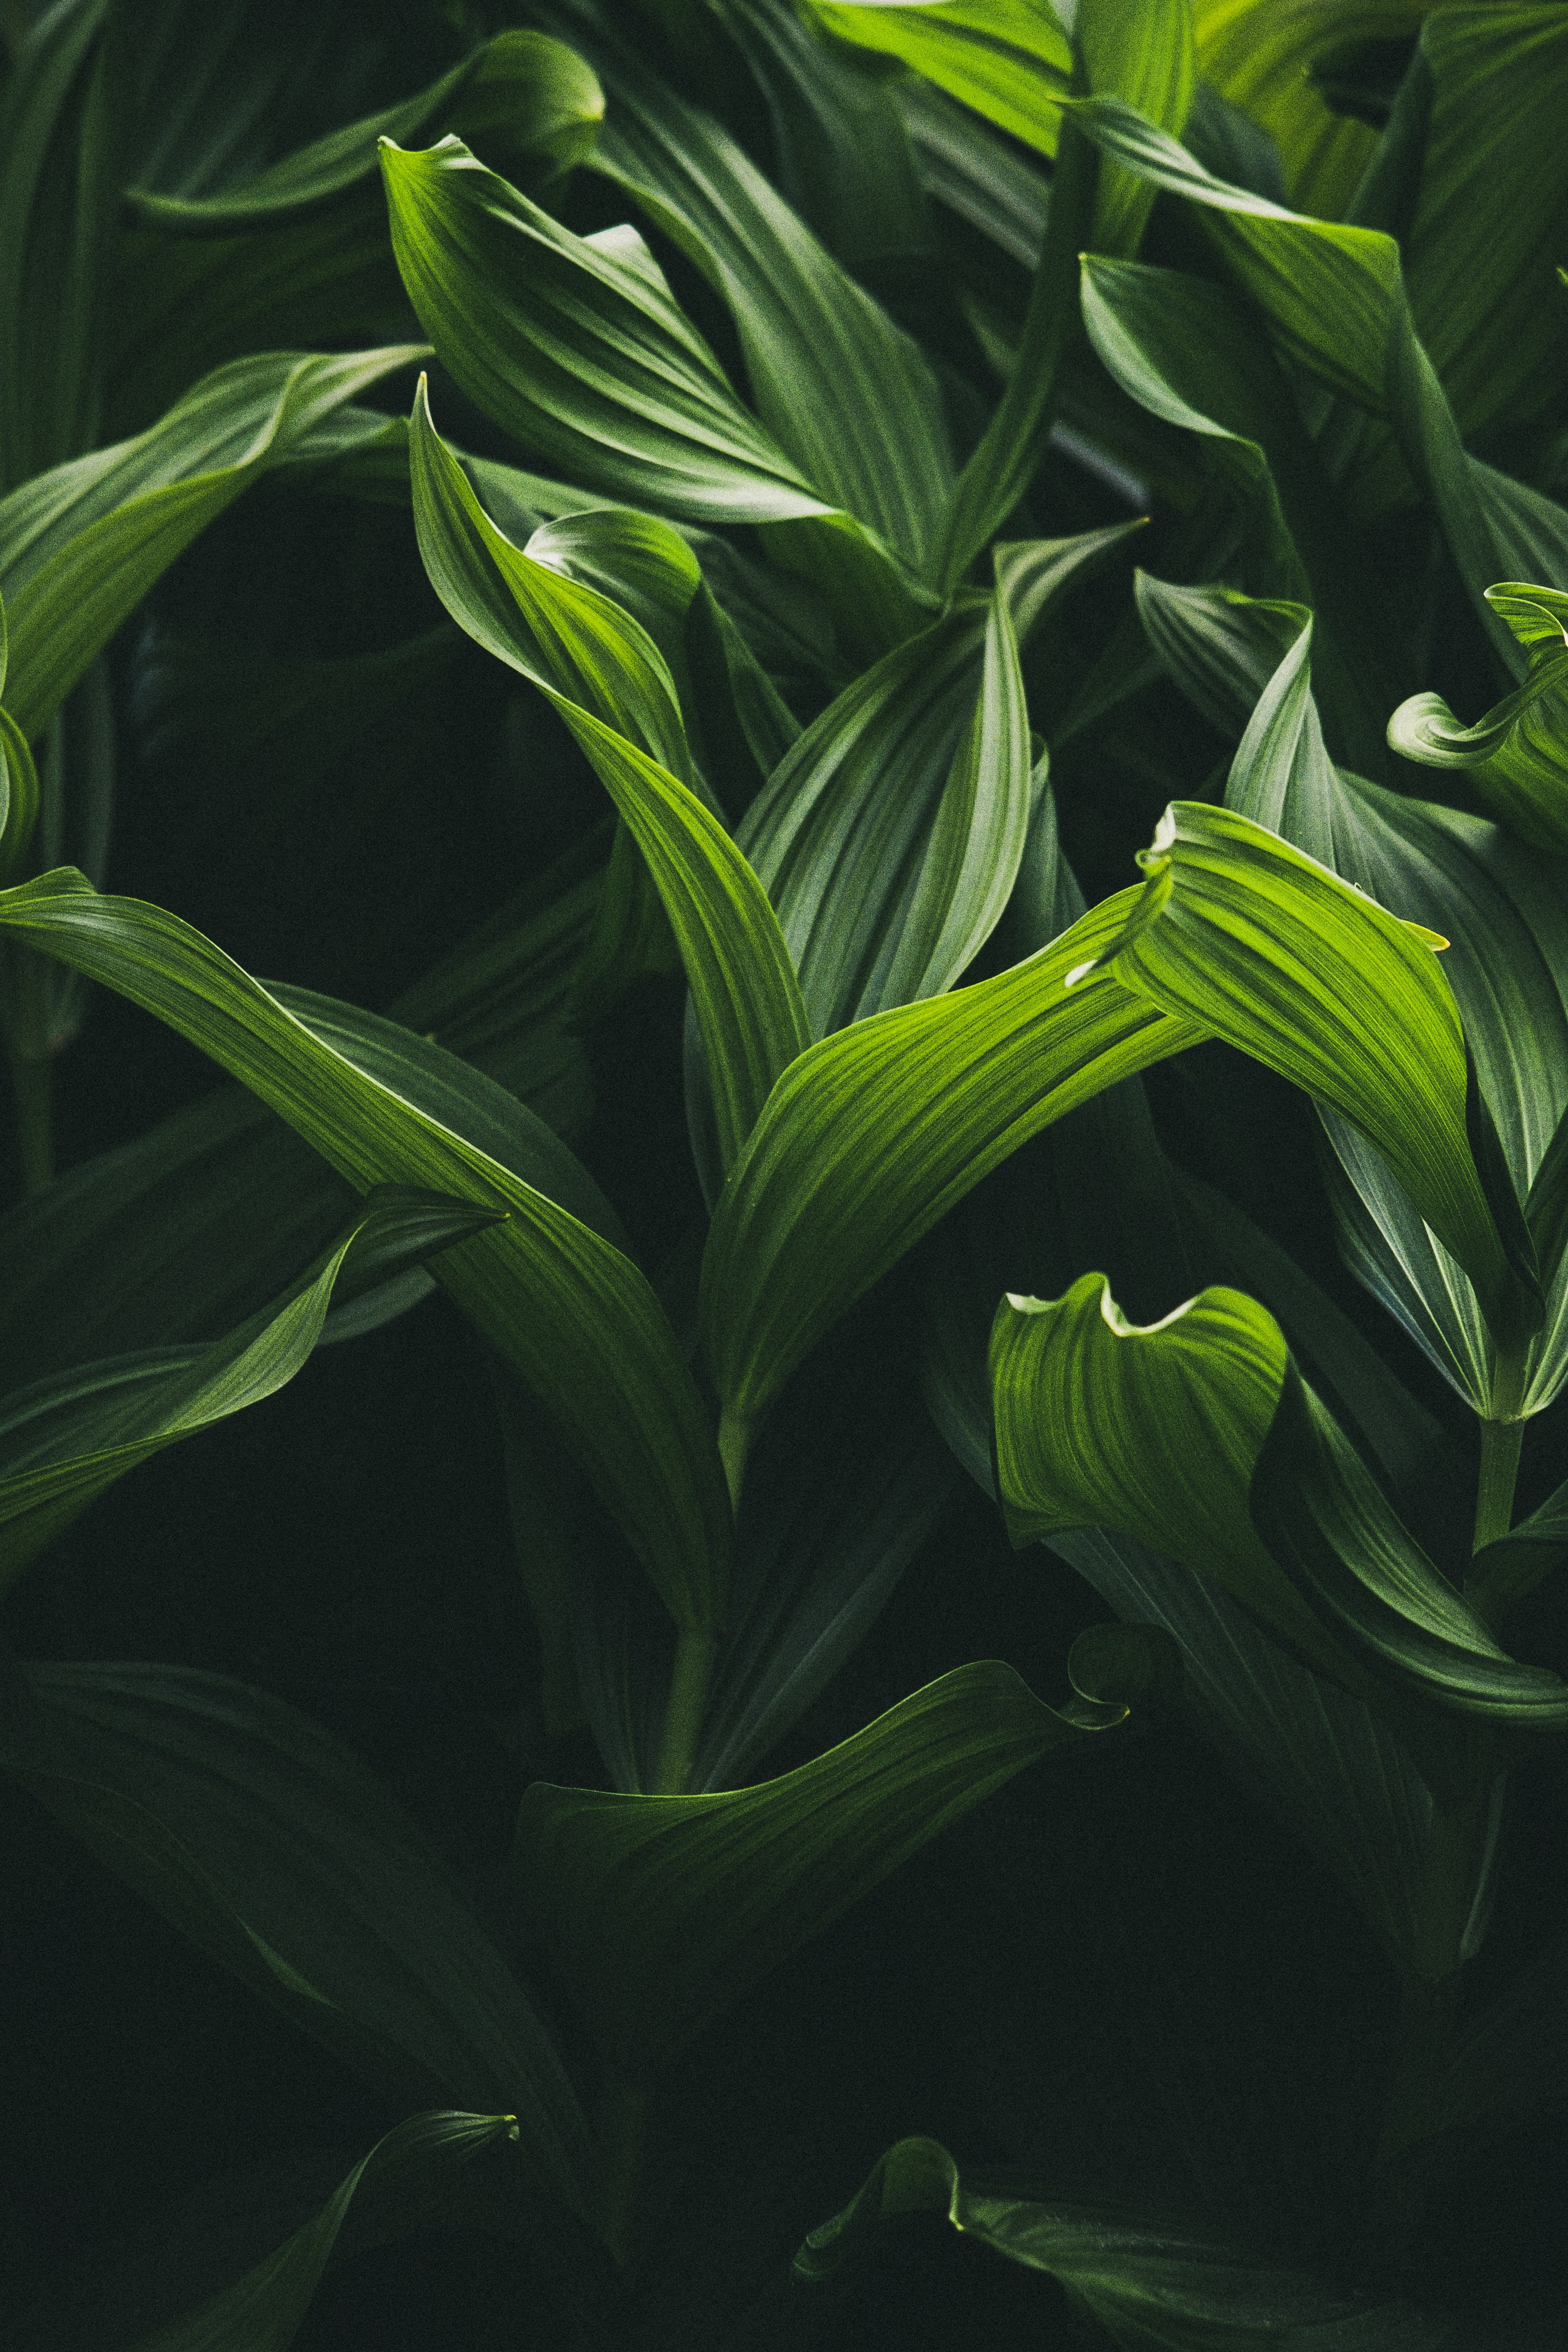
\includegraphics{13.jpg}
\end{marginfigure} 
\noindent
\large{Solution 13A}\\
Since arrangements we get by rotations are considered to be the same, we shall  first rotate the array in such a way that $1$ is placed in the first position and the rest of the $r-1$ elements wll be plced in the remaining $n-1$ slots. Let $i$ is placed in position $x_i$. Define $y_i=x_{i+1}-x_{i}-1$ for $i<r$ and $y_r=n-x_r$ \footnote{$y_i$ is supposed to be the number of available positions between $i$ and ${i+1}$ for $i<r$. For $i=r$ it is the number of available positions between $r$ and $1$}. It follows trivially that each $y_i>0$. 
Note that:
$$\sum_{i=1}^r y_i=n-x_1-(r-1)=n-1-r+1=n-r$$
The total number of solutions is $n-r-1\choose r-1$ with each solution describing one arrangement.
\begin{tcolorbox}[colback=red!5!white]
	\large{Problem 13B}\\
	Show that the following formula for binomial coefficients is a direct consequence of (10.6)
	$${n+1\choose a+b+1}=\sum_{k=0}^n{k\choose a}{n-k\choose b}$$
\end{tcolorbox}
\marginnote{Formula 10.6: $$\sum_{i=0}^\infty{a+i\choose i}x^i=\frac{1}{(1+x)^{a+1}}$$}
\large{Solution 13B}
\begin{align*}
\sum_{k=0}^n{k\choose a}{n-k\choose b}=&\sum_{k=0}^n{k\choose k-a}{n-k\choose n-k-b}\\
=&\sum_{k=0}^n{a+(k-a)\choose k-a}{b+(n-k-b)\choose n-k-b}
\end{align*}
\marginnote{For such sums where the sum is taken over all values of a parameter where the function is non-zero, we can consider the sum to be from 0 to $\infty$. This is because in cases where the sum is not defined, the terms become 0 on their own and it saves us quite a bit of bookkeeping. In this case, it would mean considering the sum to be taken from $k=0$ to $\infty$. For ore details check out the first chapter of Generatingfunctionology by Herbert Wilf}
Now,  ${a+(k-a)\choose k-a}$ is coefficient of $k-a$ in $(1-x)^{-a-1}$ and ${b+(n-k-b)\choose n-k-b}$ is coefficient of $n-k-b$ in $(1-x)^{-b-1}$. As we sum over all possible values of $k$, the sum becomes equal to the coefficient of $x^{n-a-b}$ in $(1-x)^{-(a+b+1)-1}$, which is equal to ${a++b+1+n-a-b\choose n-a-b}={n+1\choose n-a-b}={n+1\choose a+b+1}$

\begin{tcolorbox}[colback=red!5!white]
	\large{Problem 13B.5}\\
	Give a combinatorial proof of above  by considering $(a + b + 1)$-subsets of
the set $\{0, 1,\hdots,n\}$, ordering them in increasing order, and then
looking at the value of the integer in position $a + 1$.
\end{tcolorbox}\noindent
\large{Solution 13B.5}\\
Let the $a+1^{th}$ element be $k+1$. Then there are $a$ elements choosen from $1\hdots k$ which can be done in ${k\choose a}$ ways and b elements choosen from $k+2,k+3\hdots n+1$ which can be done in ${n-k}\choose b$ ways. We sum over all possible values of $a+1^{th}$ element to get all $a+b+1$ subset of $n+1$ to get the required relation.

\begin{tcolorbox}[colback=red!5!white]
	\large{Problem 13C}\\
	Give a solution involving binomial coefficients and
	a combinatorial solution to the following question. How many pairs
	$(A_1, A_2)$ of subsets of $\{1, 2,...,n\}$ are there such that $A_1 \cap A_2 = \phi$?
\end{tcolorbox}\noindent
\large{Solution 13C}\\
Each element has three choices: it either belongs to $A_1$ or $A_2$ or nither in $A_1$ or $A_2$. Therefore, the total number of pairs of $A_1,A_2$ is $3^n$.\\
We can form $A_1$ of size $r\leq n$ in $n\choose r $ ways. We can form $A_2$ from the remaining elements by taking a subset in $2^{n-r}$ ways. Therefore, we get the total number of ways to choose $A_1,A_2$ by summing over $r$
$$\sum_{r=0}^{n}{n\choose r}2^{n-r}=\sum_{r=0}^{n}{n\choose n-r}2^{n-r}=(1+2)^n=3^n$$
\begin{tcolorbox}[colback=red!5!white]
	\large{Problem 13D}\\
	Consider the set $S$ of all ordered $k$-tuples ${\mathcal A=
(A_1,...,A_k)}$ of subsets of $\{1, 2,...,n\}$. Determine
$$\sum_{\mathcal A\subseteq S}|A_1\cup A_2\hdots A_k|$$
\end{tcolorbox}\noindent
\large{Solution 13D}
We shall consider the number of ways of forming $\mathcal{A}$ so that $|A_1\cup A_2\hdots A_k|=r$. We shall use the method outlined in the book. Consider a $k\times n$ matrix $M$ with $M[ij]=1$ if $j\in A_i$ and 0 otherwise (So that the $j^{th}$ entry of $i^{th}$ row is 1 iff $j$ is present in $A_i$). Now if there are $r$ elements in $|A_1\cup A_2\hdots A_k|$ then there are exactly $n-r$ columns which are zero. The zero columns can be choosen in ${n}\choose n-r$ ways. Each of the remaining $r$ non zero columns can be filled in $2^k-1$ way.\footnote{ There are $k$ entries on each column where each entry is either $0$ or $1$ and only $1$ way to fill all of them with $0$. } Therefore total ways of forming $\mathcal A$ is ${n\choose n-r}(2^k-1)^r$. It follows that 
\begin{align*}
	\sum_{\mathcal A\subseteq S}|A_1\cup A_2\hdots A_k|=&\sum_{r=0}^n r\times\text{\# of $\mathcal{A}$ with size r}\\
	=&\sum_{r=0}^nr\times {n\choose n-r}(2^k-1)^r\\
	=&\sum_{r=0}^nr\times {n\choose r}(2^k-1)^r\\
\end{align*}
Note that:
\begin{align*}
	(1+x)^n=\sum_{r=0}^n{n\choose r}x^r\\
	\frac{d}{dx}(1+x)^n=\sum_{r=0}^n{n\choose r}\frac{d}{dx}x^r\\
	n(1+x)^{n-1}=\sum_{r=0}^n{n\choose r}rx^{r-1}\\
	nx(1+x)^{n-1}=\sum_{r=0}^n{n\choose r}rx^r\\
\end{align*}
Now set $x=2^k-1$ above to get:
$$\sum_{\mathcal A\subseteq S}|A_1\cup A_2\hdots A_k|=n(2^k-1)2^{k(n-1)}$$
\marginnote{\textbf{Taken from the hints \& answer section:} The nice closed form of the answer suggests that there is some better way to do this problem. The alternate solution is also given. I have tweaked it a bit according to my preference but the idea is the same}\\\noindent
\large{Alternate Solution:}\\
Define a function $f:S\times\mathbb{N}\to \{0,1\}$ by 
$$f(\mathcal{A},i)=\begin{cases}
	1\quad{i\in\bigcup A_j}\\
	0\quad{\text{Otherwise}}
\end{cases}$$
Note that for some $\mathcal{A}$, $|A_1\cup A_2\hdots A_k|=\sum_{i=1}^nf(\mathcal{A},i)$. Therefore, 
$$\sum_{\mathcal A\subseteq S}|A_1\cup A_2\hdots A_k|=\sum_{\mathcal A\subseteq S}\sum_{i=1}^nf(\mathcal{A},i)=\sum_{i=1}^n\sum_{\mathcal A\subseteq S}f(\mathcal{A},i)$$
$\sum_{\mathcal A\subseteq S}f(\mathcal{A},i)$ means number of $\mathcal{A}$ such that $i$ is contained in the union. We now use $M$ as defined above. As $i$ is contained in the union, the $i^{th}$ column filled with 0's and 1's in $2^{k}-1$ ways. The remaining $k\times (n-1)$ entries can be filled in $2^{k(n-1)}$ ways. Therefore, $\sum_{\mathcal A\subseteq S}f(\mathcal{A},i)=(2^k-1)2^{k(n-1)}$ and  
$$\sum_{\mathcal A\subseteq S}|A_1\cup A_2\hdots A_k|=n(2^k-1)2^{k(n-1)}$$


\begin{tcolorbox}[colback=red!10!white]
	\large{Problem 13E}\\
	The familiar relation
	$$\sum_{m=k}^l{m\choose k}={l+1\choose k+1}$$
	Find a combinatorial proof
by counting paths from $(0,0)$ to $(l+1, k+1)$ in the X-Y plane where
each step is of type $(x, y) \to (x + 1, y)$ or $(x, y) \to (x + 1, y + 1)$.
Then use the formula to show that the number of solutions of
$$x_1+x_2+x_3\hdots +x_k\leq n$$
in nonnegative integers is $n+k\choose k$
. Can you prove this result combinatorially?
\end{tcolorbox}






\begin{tcolorbox}[colback=blue!10!white]
	\large{Problem 13F}\\
	Show directly that the number of permutations of
the integers 1 to $n$ with an even number of cycles is equal to the
number of permutations with an odd number of cycles $(n > 1)$.
Also show that this is a consequence of Theorem 13.7.
\end{tcolorbox}
\large{Solution 13F}\\
This is true for $n=2$. Assume it is true for $N=n$. Let number of permutation with odd cycles for integers 1 to $n$ be $O(n)$ and number of permutation with even integers be $E(n)$. Consider permutations of integers from 1 to $N=n+1$ with an even number of cycles. There are 2 cases possible:
\begin{enumerate}
	\item $n+1$ forms an cycle by itself( i.e $\sigma(n+1)=n+1$): Then the remaining $n$ elements form an permutation anong themselves with an odd number of cycles. 
	\item $n+1$ is not in a cycle by itself: Write down the pemutation in cyclic notation\footnote{Check Artin's Algebra for details}. Note that removing $n+1$ gives a permutation of $n$ elements with an even number of cycles. Conversely, given a  permutation of $n$ elements with an even number of cycles, there are $n$ places to Insert a new element $n+1$ to form a permutation of $n+1$ elements. 
\end{enumerate} 
Therefore we have:
$$E(n+1)=O(n)+nE(n)$$
and similarly:
$$O(n+1)=E(n)+nO(n)$$
Therefore, we get:  $E(n+1)-O(n+1)=n\left(E(n)-O(n)\right)=0$. Therefore, the statement is true by induction.






\backmatter


\bibliography{sample-handout}
\bibliographystyle{plainnat}


\end{document}

